\documentclass[a4paper]{report}\usepackage[]{graphicx}\usepackage[]{color}
%% maxwidth is the original width if it is less than linewidth
%% otherwise use linewidth (to make sure the graphics do not exceed the margin)
\makeatletter
\def\maxwidth{ %
  \ifdim\Gin@nat@width>\linewidth
    \linewidth
  \else
    \Gin@nat@width
  \fi
}
\makeatother

\definecolor{fgcolor}{rgb}{0.345, 0.345, 0.345}
\newcommand{\hlnum}[1]{\textcolor[rgb]{0.686,0.059,0.569}{#1}}%
\newcommand{\hlstr}[1]{\textcolor[rgb]{0.192,0.494,0.8}{#1}}%
\newcommand{\hlcom}[1]{\textcolor[rgb]{0.678,0.584,0.686}{\textit{#1}}}%
\newcommand{\hlopt}[1]{\textcolor[rgb]{0,0,0}{#1}}%
\newcommand{\hlstd}[1]{\textcolor[rgb]{0.345,0.345,0.345}{#1}}%
\newcommand{\hlkwa}[1]{\textcolor[rgb]{0.161,0.373,0.58}{\textbf{#1}}}%
\newcommand{\hlkwb}[1]{\textcolor[rgb]{0.69,0.353,0.396}{#1}}%
\newcommand{\hlkwc}[1]{\textcolor[rgb]{0.333,0.667,0.333}{#1}}%
\newcommand{\hlkwd}[1]{\textcolor[rgb]{0.737,0.353,0.396}{\textbf{#1}}}%

\usepackage{framed}
\makeatletter
\newenvironment{kframe}{%
 \def\at@end@of@kframe{}%
 \ifinner\ifhmode%
  \def\at@end@of@kframe{\end{minipage}}%
  \begin{minipage}{\columnwidth}%
 \fi\fi%
 \def\FrameCommand##1{\hskip\@totalleftmargin \hskip-\fboxsep
 \colorbox{shadecolor}{##1}\hskip-\fboxsep
     % There is no \\@totalrightmargin, so:
     \hskip-\linewidth \hskip-\@totalleftmargin \hskip\columnwidth}%
 \MakeFramed {\advance\hsize-\width
   \@totalleftmargin\z@ \linewidth\hsize
   \@setminipage}}%
 {\par\unskip\endMakeFramed%
 \at@end@of@kframe}
\makeatother

\definecolor{shadecolor}{rgb}{.97, .97, .97}
\definecolor{messagecolor}{rgb}{0, 0, 0}
\definecolor{warningcolor}{rgb}{1, 0, 1}
\definecolor{errorcolor}{rgb}{1, 0, 0}
\newenvironment{knitrout}{}{} % an empty environment to be redefined in TeX

\usepackage{alltt}
\usepackage[utf8]{inputenc}
\usepackage[T1]{fontenc}
\usepackage{RJournal_edited}
\usepackage{amsmath,amssymb,array,float,subcaption}
\usepackage{booktabs}
%\VignetteIndexEntry{Introduction to rotations}
%\VignetteDepends{knitr}
%\VignetteEngine{knitr::knitr}

%% load any required packages here
\usepackage{bm,subcaption,amsfonts}
\IfFileExists{upquote.sty}{\usepackage{upquote}}{}
\begin{document}


%% do not edit, for illustration only
\sectionhead{}
\volume{}
\volnumber{}
\year{}
\month{}
\begin{article}
%% replace RJtemplate with your article
\title{Extending the capabilities of agriculture simulators using R, an introduction to the \pkg{apsimr} package}
\author{by Bryan Stanfill}

\maketitle
\end{article}

\section{Introduction}

The {\bf A}gricultural {\bf P}roduction {\bf S}ystem s{\bf IM}ulator (APSIM) is a widely used, powerful and highly complex computer program \citep{keating2003overview, holzworth2014apsim}.  Based on information about weather, soil properties, farming practices and land use, APSIM can predict crop and environmental outcomes such as yield, nitrogen runoff and sediment loss as a function of time and space.  

APSIM is currently run either from a clunky and unappealing user interface (Figure \ref{fig:UI}) with limited analysis and visualization tools available, or from the command line, whic requires a high level of familiarity with APSIM and a substantial amount of ad hoc programming.  The \CRANpkg{apsimr} package includes functions to create, edit, run and analyze APSIM simulations using R.  Additionally, \pkg{apsimr} acts as a bridge between the \CRANpkg{sensitivity} package and APSIM, which provides APSIM users with access to a wide variety of uncertainty quantification tools \citep{pujol2014sensitivity}.  Other packages that could be of interest for uncertainty/sensitivity analysis of APSIM are \CRANpkg{spartan} and \CRANpkg{multisensi} \citep{alden2014applying,lamboni2011multivariate}.

\begin{figure}[h]
\centering
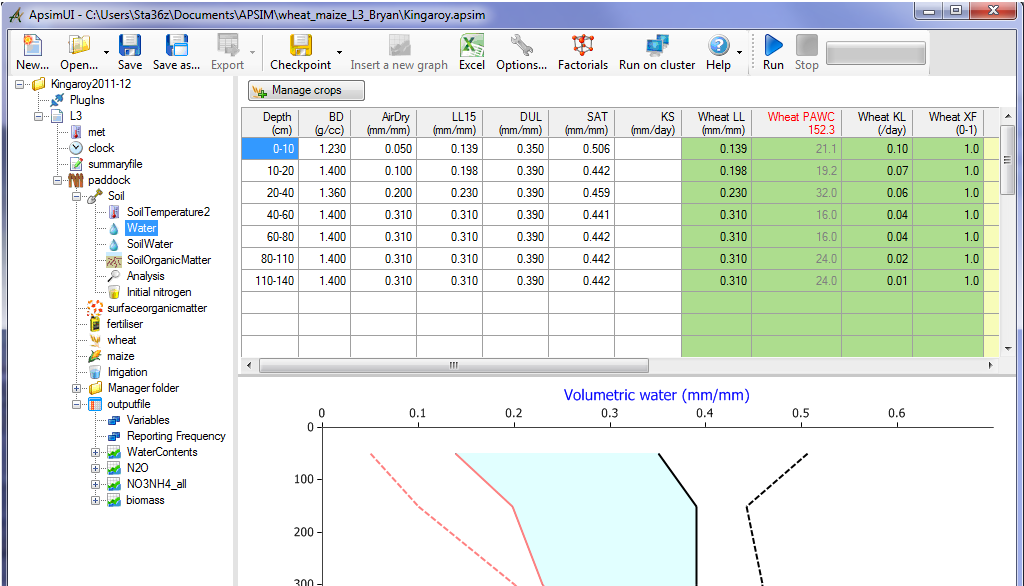
\includegraphics[width=.9\textwidth]{figures/APSIMUI.png}
\caption{The user interface for APSIM version 7.6.}
\label{fig:UI}
\end{figure}

In the remainer of this vignette I give a general overview of APSIM then explain how the \pkg{apsimr} package can be used to run, edit, visualize and analyze APSIM using R.

\section{APSIM Overview}

This section gives a brief account of how APSIM works because it will inform the construction of the package.  For a detailed description see \cite{keating2003overview}, or \cite{holzworth2014apsim} and the references therein.

APSIM is composed of several independent modules, each of which controls a specific apsect of the simulation.  Modules control everything, including crop growth, soil water balance, soil nitrogen levels, and farming practices (e.g.~how much fertilizer to apply and when).  Crop growth statistics are produced for each day in the simulation and are determined by daily weather information, soil characteristics and management choices.  The weather data is provided by the user in the form of a \verb=.met= file.  Soil characteristics and management choices are controlled by the soil and management modules, respectively.


Each module relies on a separate \verb=.xml= file for instructions including parameter values.  The module \verb=.xml= files can have any name, but are often titled \verb=Soil.xml=, \verb=Wheat.xml= or something similar.  These separate \verb=.xml= files are called by the \verb=.apsim= file, which controls the entire simulation.  Note that \verb=.apsim= files are also simple \verb=.xml= files with a different extension.  The simulation file controls the simulation metadata, such as what outputs to report, how often to report those outputs, where to find the module files and where to write the results file.  

Every APSIM simulation run will produce a text file with the file extension \verb=.sum=, which contains a detailed summary of the simulation including possible errors.  When an APSIM simulation has run successfully, an additional text file with the extension \verb=.out= is written, which contains the specifed outcomes at the specified time steps.  The user can specify the file names as well as where the files are written.  By default, both files inheret the name of the simulation and are written in the same directory as the run simulation.  For example, if no output name or location is specified by the user then the results of the simulation \verb=Millet.apsim= currently stored on the user's desktop, then APSIM will create files \verb=Millet.sum= and \verb=Millet.out= on the user's desktop. 

\section{Running APSIM}

The function used to run APSIM from R is called \code{apsim}.  Its only required argument is \code{exe}, which is the path to the APSIM executable file on your machine.  Additional arguments include  \code{wd} and \code{files}.  The \code{wd} argument specifies the working directory to which the results will be written and is set to the current working directory by default.  The argument \code{files} is the list of \verb=.apsim= simulation files to be run, which is set to all \verb=.apsim= files in the specified working directory by default.
\begin{knitrout}
\definecolor{shadecolor}{rgb}{0.969, 0.969, 0.969}\color{fgcolor}\begin{kframe}
\begin{alltt}
\hlstd{apsimExe} \hlkwb{<-}\hlstr{"C:/Program Files (x86)/Apsim75-r3008/Model/Apsim.exe"}
\hlstd{apsimWd} \hlkwb{<-} \hlstr{"~/APSIM"}
\hlstd{to_run} \hlkwb{<-} \hlkwd{c}\hlstd{(}\hlstr{"Canopy.apsim"}\hlstd{,} \hlstr{"Continuous Wheat.apsim"}\hlstd{)}
\hlstd{results} \hlkwb{<-} \hlkwd{apsim}\hlstd{(}\hlkwc{exe} \hlstd{= apsimExe,} \hlkwc{wd} \hlstd{= apsimWd,} \hlkwc{files} \hlstd{= to_run)}
\end{alltt}
\end{kframe}
\end{knitrout}


\section{Editing APSIM}

The file I want to edit is called "Canopy.apsim" which is in the directory "$\sim$/APSIM"
\begin{knitrout}
\definecolor{shadecolor}{rgb}{0.969, 0.969, 0.969}\color{fgcolor}\begin{kframe}
\begin{alltt}
\hlstd{apsimFile} \hlkwb{<-} \hlstr{"Canopy.apsim"}
\hlstd{apsimWd} \hlkwb{<-} \hlstr{"~/APSIM"}
\end{alltt}
\end{kframe}
\end{knitrout}
I want to change the Thickness of the Soilwater, the SoilCN of the SoilOrganicMatter and the state at which the simulation is being run.
Change SoilWater-Thickness to 200,200,300$\times$9
Change SoilCN to 10

\begin{knitrout}
\definecolor{shadecolor}{rgb}{0.969, 0.969, 0.969}\color{fgcolor}\begin{kframe}
\begin{alltt}
\hlstd{var} \hlkwb{<-} \hlkwd{c}\hlstd{(}\hlstr{"SoilWater/Thickness"}\hlstd{,} \hlstr{"SoilOrganicMatter/SoilCN"}\hlstd{)}
\hlstd{value} \hlkwb{<-} \hlkwd{list}\hlstd{(}\hlkwd{c}\hlstd{(}\hlkwd{rep}\hlstd{(}\hlnum{200}\hlstd{,} \hlnum{2}\hlstd{),} \hlkwd{rep}\hlstd{(}\hlnum{300}\hlstd{,} \hlnum{9}\hlstd{)),} \hlnum{10}\hlstd{)}
\end{alltt}
\end{kframe}
\end{knitrout}

The next snippit edits the apsim file without overwriting it.  This results in the new file being written into the \code{wd} with the additional tage "-updated.apsim".  In this case the new file "Canopy-edited.apsim" is identical to "Canopy.apsim" except for the variables that have been changed by the above code snippet.  If the option \code{overwrite=TRUE} then "Canopy.apsim" is overwritten with the new variable values.
\begin{knitrout}
\definecolor{shadecolor}{rgb}{0.969, 0.969, 0.969}\color{fgcolor}\begin{kframe}
\begin{alltt}
\hlkwd{edit_apsim}\hlstd{(apsimFile, apsimWd, var, value,} \hlkwc{overwrite} \hlstd{=} \hlnum{FALSE}\hlstd{)}
\end{alltt}
\end{kframe}
\end{knitrout}

\section{Beyond the Conventional}

\subsection{Advanced Visualizations}

Visualize all of the results as a function of time in separate plots
\begin{knitrout}
\definecolor{shadecolor}{rgb}{0.969, 0.969, 0.969}\color{fgcolor}\begin{kframe}
\begin{alltt}
\hlkwd{plot}\hlstd{(results[[}\hlnum{2}\hlstd{]],} \hlkwc{geom} \hlstd{=} \hlstr{'line'}\hlstd{)}
\end{alltt}
\end{kframe}
\end{knitrout}

Put all variables on one faceted plot (Figure \ref{fig:allon1}).
\begin{knitrout}
\definecolor{shadecolor}{rgb}{0.969, 0.969, 0.969}\color{fgcolor}\begin{kframe}
\begin{alltt}
\hlkwd{plot}\hlstd{(results[[}\hlnum{2}\hlstd{]],} \hlkwc{one_plot} \hlstd{=} \hlnum{TRUE}\hlstd{,} \hlkwc{geom} \hlstd{=} \hlstr{'line'}\hlstd{)} \hlopt{+} \hlkwd{theme_bw}\hlstd{()}
\end{alltt}
\end{kframe}
\end{knitrout}

\begin{figure}[H]
\centering
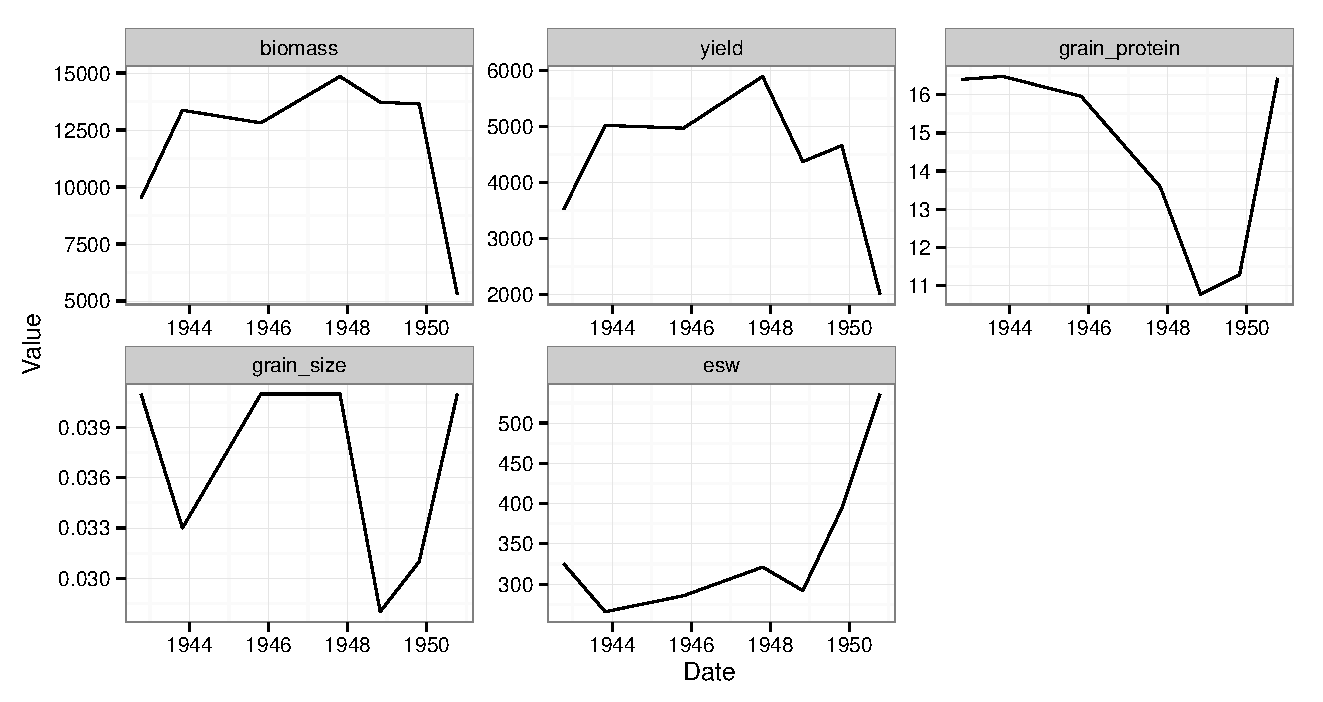
\includegraphics[width=1\textwidth]{figures/allon1}
\caption{Figures produced by \code{plot.apsim} with argument \code{one\_plot = TRUE}.}
\label{fig:allon1}
\end{figure}

Plot just yield as a function of time (Figure \ref{fig:yield}).
\begin{knitrout}
\definecolor{shadecolor}{rgb}{0.969, 0.969, 0.969}\color{fgcolor}\begin{kframe}
\begin{alltt}
\hlkwd{plot}\hlstd{(results[[}\hlnum{2}\hlstd{]],} \hlkwc{y} \hlstd{=} \hlstr{'yield'}\hlstd{)} \hlopt{+} \hlkwd{geom_line}\hlstd{(}\hlkwc{colour} \hlstd{=} \hlstr{'red'}\hlstd{)} \hlopt{+} \hlkwd{theme_bw}\hlstd{()}
\end{alltt}
\end{kframe}
\end{knitrout}

\begin{figure}[H]
\centering
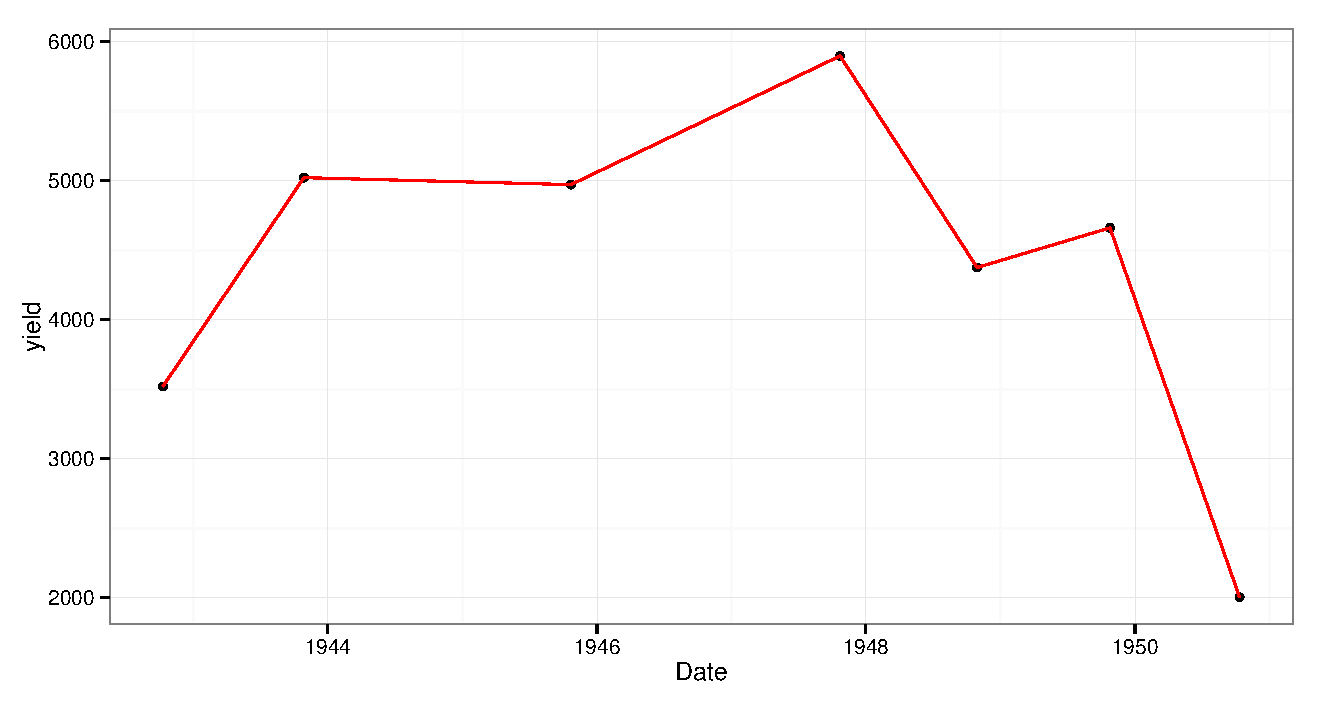
\includegraphics[width=1\textwidth]{figures/yield}
\caption{Plot produced by \code{plot.apsim} with argument \code{y = 'yield'}.}
\label{fig:yield}
\end{figure}


\subsection{Sensitivity Analysis}

The function \code{apsim\_sen} is a version of \code{apsim} that has been adapted so it can be used with the package \CRANpkg{sensitivity}.  In particular, the function \code{apsim} returns a data frame that includes different outputs over the specified time frame at specified time intervals.  The \code{apsim\_sen} function takes and argument \code{g} that translates the output of \code{apsim} into a single, univaraite outcome.  This way, the function \code{apsim\_sen} can be passed to functions in the \code{sensitivity} package as the \code{model} argument.  

Below is an example of a \code{g} function and how sensitivity analysis of APSIM can be accomplished.  First, load the sensitivity package and define a \code{g} function.  In this example we are interested in how sensitive the average cowpea yield is to initial values in the soil organic matter and soil water.  Therefore we define the \code{g} function so that the average cowpea yield is returned everytime APSIM is executed.  We define the  three inputs of interest in the \code{vars} argument: the soil organic matters soil carbon (\code{SoiCN}), the soilwaters diffuse constant (\code{DiffusConst}) and the carbon-nitrogen covariance (\code{CNCov}).  

The \pkg{sensitivity} package includes several methods to perform sensitivity analysis.  For this example we chose the \code{soboljansen} function which estimates first and total Sobol' indices as described in \cite{saltelli2010variance}. The \code{soboljansen} function requires two data frames, \code{X1} and \code{X2}, to define the points in the input space at which to run the \code{model}.  The function in the \pkg{apsimr} package to use for sensntivity analysis is \code{apsim\_sen}, therefore we set \code{model=apsim\_sen}.  We define the \code{X1} and \code{X2} matrices so that each variable is an independent uniform random variable on an appropriate interval.  The \code{soboljansen} function allows for additional arguments to be passed to the \code{model} argument.  The function \code{apsim\_sen} requires the following additional arguments: the APSIM executable location \code{exe}, the working directory to find the .apsim file to run \code{wd}, and if the edits .apsim file should be overwritten or not \code{overwrite}.  The results of this sensitivity analysis are give in Figure \ref{fig:soboljansen}, which was produced by the \code{print} routine for the outputs from the \code{soboljansen}.  \emph{Note:} the function \code{soboljansen} requires $p\times n$ model evaluations, where $n$ is a user specified number of model evaluations (500 below) and $p$ is the number of input parameter considered (3 below).

\begin{knitrout}\footnotesize
\definecolor{shadecolor}{rgb}{0.969, 0.969, 0.969}\color{fgcolor}\begin{kframe}
\begin{alltt}
\hlkwd{library}\hlstd{(sensitivity)}

\hlstd{meanYield}\hlkwb{<-}\hlkwa{function}\hlstd{(}\hlkwc{x}\hlstd{)\{}
  \hlkwd{return}\hlstd{(}\hlkwd{mean}\hlstd{(x}\hlopt{$}\hlstd{lai_cowpea))}
\hlstd{\}}

\hlstd{vars} \hlkwb{<-} \hlkwd{c}\hlstd{(}\hlstr{"SoilOrganicMatter/SoilCN"}\hlstd{,} \hlstr{"SoilWater/DiffusConst"}\hlstd{,} \hlstr{"SoilWater/CNCov"}\hlstd{)}

\hlstd{n} \hlkwb{<-} \hlnum{20}
\hlstd{X1} \hlkwb{<-} \hlkwd{data.frame}\hlstd{(}\hlkwc{SoilCN} \hlstd{=} \hlkwd{runif}\hlstd{(n,} \hlnum{5}\hlstd{,} \hlnum{25}\hlstd{),}
                 \hlkwc{DiffusConst} \hlstd{=} \hlkwd{runif}\hlstd{(n,} \hlnum{20}\hlstd{,} \hlnum{50}\hlstd{),} \hlkwc{CNCov} \hlstd{=} \hlkwd{runif}\hlstd{(n,} \hlnum{0}\hlstd{,} \hlnum{1}\hlstd{))}
\hlstd{X2} \hlkwb{<-} \hlkwd{data.frame}\hlstd{(}\hlkwc{SoilCN} \hlstd{=} \hlkwd{runif}\hlstd{(n,} \hlnum{5}\hlstd{,} \hlnum{25}\hlstd{),}
                 \hlkwc{DiffusConst} \hlstd{=} \hlkwd{runif}\hlstd{(n,} \hlnum{20}\hlstd{,} \hlnum{50}\hlstd{),} \hlkwc{CNCov} \hlstd{=} \hlkwd{runif}\hlstd{(n,} \hlnum{0}\hlstd{,} \hlnum{1}\hlstd{))}

\hlstd{sobolResults} \hlkwb{<-} \hlkwd{soboljansen}\hlstd{(}\hlkwc{model} \hlstd{= apsim_vector, X1, X2,} \hlkwc{exe} \hlstd{= apsimExe,} \hlkwc{wd} \hlstd{= apsimWd,}
                        \hlkwc{vars} \hlstd{= vars,} \hlkwc{to.run} \hlstd{= apsimFile,} \hlkwc{g} \hlstd{= meanYield,} \hlkwc{overwrite} \hlstd{=} \hlnum{TRUE}\hlstd{)}
\hlkwd{plot}\hlstd{(sobolResults)}
\end{alltt}
\end{kframe}
\end{knitrout}


\begin{figure}[H]
\centering
\begin{subfigure}[b]{1\textwidth}
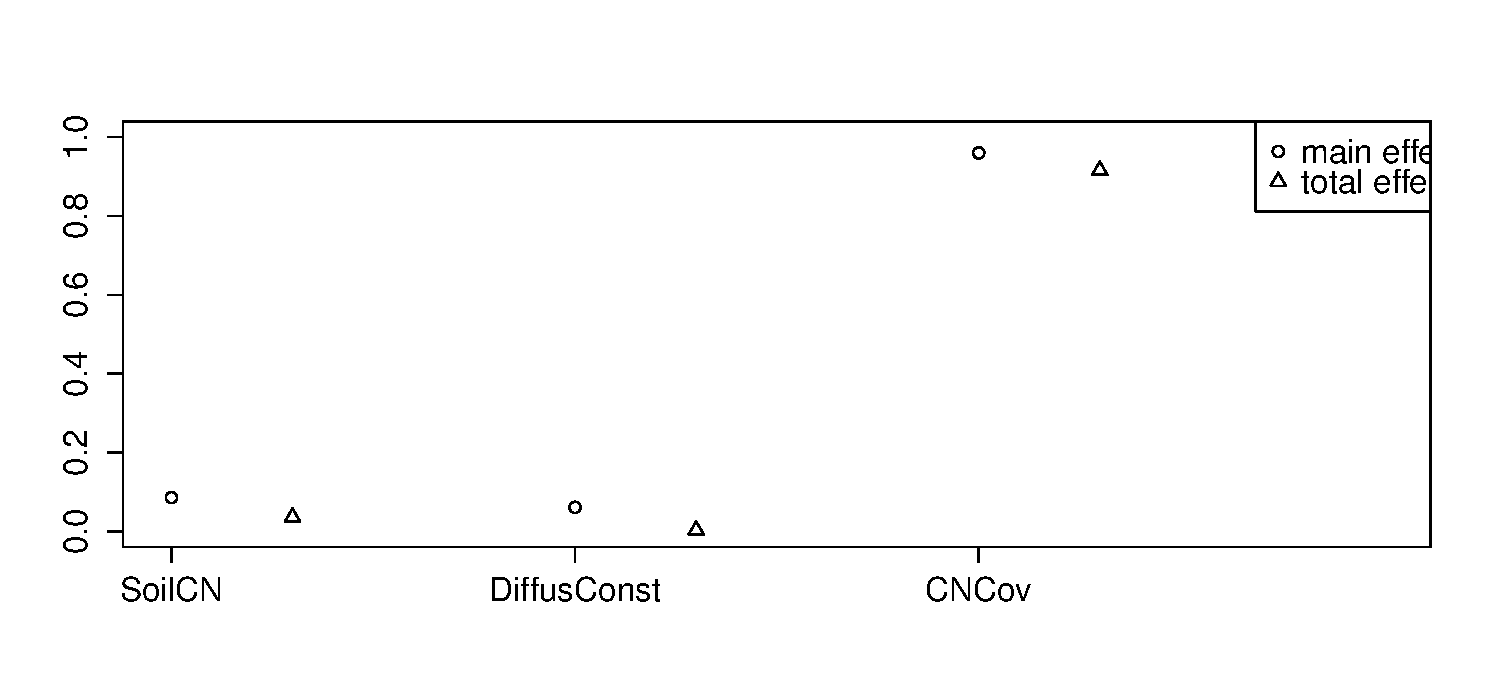
\includegraphics[width=\textwidth]{figures/soboljan.pdf}%\vspace{-2.5em}
\caption{Index estimates using \code{soboljansen} function.}
\label{fig:soboljansen}
\end{subfigure}

\begin{subfigure}[b]{1\textwidth}
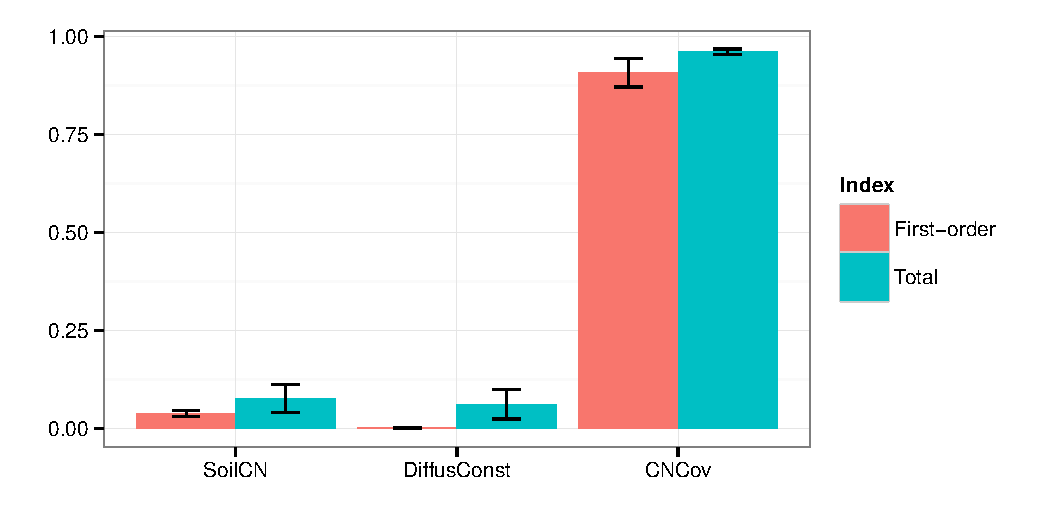
\includegraphics[width=\textwidth]{figures/emulRespic.pdf}%\vspace{-2.5em}
\caption{Index estimates using \code{SAemulator} function with \code{method = "singleGAM"}}
\label{fig:SAemulator}
\end{subfigure}%\vspace{-1em}
\caption{The results of the sensitivity analysis of the APSIM Canopy simulation for the average cowpea yield over time.}
\label{fig:yield}
\end{figure}


An alternative, and potentially more efficient, method for sensitivity analysis is via emulators.  The function \code{SAemulator} estimates sensitivity indices for each input (column of \code{X}) for the computer program \code{model}.  If computer model runs corresponding to the input matrix \code{X} are available then the one can forgo the \code{model} argument and include the computer model runs with the \code{y} argument.  \empg{Note:} the \code{y} argument takes precidence over the \code{model} argument and an error is returned if the number of rows in \code{X} does not match the length of \code{y}.  

There are two methods to emulating the \code{model}: a single GAM emulation method or a separate GAM method differentiated by \code{method = "singleGAM"} and \code{method = "separateGAM"}, respecitvely.  Data frames consisting of first-order and total sensitivity index estimates along with a standard error, bias, lower and upper confidence bounds are returned along with the fitted means and residuals for each fitted model to assess model assumptions such as homoscedasticity.  The separate GAM method cannot be used to estimate the total sensitivity indices, but the single GAM method can.  

The \code{SAemulator} function returns an object of class \code{"gamSA"}, which has its own plotting routine included in the package.  The example code below demonstrates how to call the \code{SAemulator} function and plot the results of the \code{method = "singleGAM"} option.  Figure \ref{fig:SAemulator} is the result of \code{plot(emulRes)} using the \code{ggplot2} functionality.  Note that atleast $8p^2-4p+1$ model runs are required to fit the single GAM where $p$ is the number of parameters included in the.

\begin{knitrout}\footnotesize
\definecolor{shadecolor}{rgb}{0.969, 0.969, 0.969}\color{fgcolor}\begin{kframe}
\begin{alltt}
\hlstd{emulRes} \hlkwb{<-} \hlkwd{apsim_emul_sa}\hlstd{(}\hlkwc{model} \hlstd{= apsim_vector,} \hlkwc{X} \hlstd{= X1,} \hlkwc{method} \hlstd{=} \hlstr{"singleGAM"}\hlstd{,} \hlkwc{exe} \hlstd{= apsimExe,} \hlkwc{wd} \hlstd{= apsimWd,}
                        \hlkwc{vars} \hlstd{= vars,} \hlkwc{to.run} \hlstd{= apsimFile,} \hlkwc{g} \hlstd{= meanYield,} \hlkwc{overwrite} \hlstd{=} \hlnum{TRUE}\hlstd{)}
\hlkwd{plot}\hlstd{(emulRes)}
\end{alltt}
\end{kframe}
\end{knitrout}

The ability to simply include model runs instead of the model itself sets the \code{SAemulator} is a crucial difference between it and the sensitivity analysis functions in \pkg{sensitivity}.  This crucial difference makes multivariate global sensitivity analysis of APSIM possible because the basis functions of the APSIM runs can be passed with the \code{y} argument.  See \cite{campbell2006sensitivity} for more about multivariate global sensitivity analysis. 

\begin{knitrout}\footnotesize
\definecolor{shadecolor}{rgb}{0.969, 0.969, 0.969}\color{fgcolor}\begin{kframe}
\begin{alltt}
\hlstd{rawYield} \hlkwb{<-} \hlkwa{function}\hlstd{(}\hlkwc{x}\hlstd{)\{}
  \hlkwd{return}\hlstd{(x}\hlopt{$}\hlstd{cowpea.yield)}
\hlstd{\}}

\hlstd{cowpeaY} \hlkwb{<-} \hlkwd{apsim_vector}\hlstd{(}\hlkwc{X} \hlstd{= X1,} \hlkwc{exe} \hlstd{= apsimExe,} \hlkwc{wd} \hlstd{= apsimWd,} \hlkwc{vars} \hlstd{= vars,} \hlkwc{toRun} \hlstd{= apsimFile,} \hlkwc{g} \hlstd{= rawYield,} \hlkwc{overwrite} \hlstd{=} \hlnum{TRUE}\hlstd{)}

\hlstd{vCowpea}\hlkwb{<-}\hlkwd{var}\hlstd{(cowpeaY)}
\hlstd{pcsY}\hlkwb{<-}\hlkwd{svd}\hlstd{(vCowpea)}\hlopt{$}\hlstd{u}
\hlstd{N}\hlkwb{<-}\hlkwd{nrow}\hlstd{(cowpeaY)}
\hlstd{ones}\hlkwb{<-}\hlkwd{matrix}\hlstd{(}\hlkwd{rep}\hlstd{(}\hlnum{1}\hlstd{,N),}\hlkwc{ncol}\hlstd{=}\hlnum{1}\hlstd{)}
\hlstd{yBar}\hlkwb{<-}\hlstd{(}\hlnum{1}\hlopt{/}\hlstd{N)}\hlopt{*}\hlstd{ones}\hlopt\hlkwd{t}\hlstd{(ones)}\hlopt\hlstd{cowpeaY}
\hlstd{cowpeaPCS}\hlkwb{<-}\hlstd{(cowpeaY}\hlopt{-}\hlstd{yBar)}\hlopt\hlstd{pcsY}

\hlstd{mgsaRes} \hlkwb{<-} \hlkwd{vector}\hlstd{(}\hlstr{"list"}\hlstd{,}\hlnum{5}\hlstd{)}

\hlkwa{for}\hlstd{(i} \hlkwa{in} \hlnum{1}\hlopt{:}\hlnum{5}\hlstd{)\{}
  \hlstd{mgsaRes[[i]]} \hlkwb{<-} \hlkwd{SAemulator}\hlstd{(}\hlkwc{y} \hlstd{= cowpeaPCS[,i],} \hlkwc{X} \hlstd{= X1,} \hlkwc{method} \hlstd{=} \hlstr{"separateGAM"}\hlstd{)}
\hlstd{\}}
\end{alltt}
\end{kframe}
\end{knitrout}


\bibliography{apsimr_refs}

\end{document}
